%% the following is necessary for using colours in tabular
\PassOptionsToPackage{table}{xcolor}
\documentclass[pdf]{beamer}
\mode<presentation>{}
\usepackage{minted}
\usepackage{tikz}
\usepackage{pgffor} %% gives looping with \foreach
\usepackage[absolute,overlay]{textpos}
\usepackage{lmodern} %% scalable latin characters
\usetikzlibrary{arrows,shapes,backgrounds}
\usepackage{multirow}
\usepackage{tabu}
\usepackage[utf8]{inputenc}

%% it seems that beamer and descriptions can be a bit
%% tricky, so we need to define some things ourselves
\defbeamertemplate{description item}{align left}{\insertdescriptionitem\hfill}

%% I detest indentation in footnotes etc, so try this:
\makeatletter
\renewcommand\@makefntext[1]{\noindent\makebox[0em][r]{\@makefnmark}\tiny#1}
\makeatother
%% the makeatletter and makeatother are required to allow me to
%% to change the macro beginning with an @. (though when I call it
%% I don't use the @ ... 


\title{Course Introduction}
\subtitle{Introduction to B1229F 2015}
\author{Martin Jakt}

%% a command to define a subheading
\newcommand\subHeading[1]{
  \par\bigskip {\Large\bfseries#1}\par\smallskip
}

\setlength{\parskip}{0.5em}

\begin{document}

\begin{frame}
  \titlepage
\end{frame}

\begin{frame}{Course structure}
  \begin{itemize}
    \item 19 $x$ 1 hr 45 minute sessions.
    \pause
    \item 45 min. lecture $\rightarrow$ 15 min. break $\rightarrow$ 45 min. discussion
    \pause
    \item $\sim$4 (3 hour) practical computer sessions
    \pause
    \item Introductory level (nothing really complicated)
  \end{itemize}
  \pause
  Content will be adjusted as we progress.\\
  Suggestions for changes to format and content are welcome.
\end{frame}

\begin{frame}{Reference Material}
  \begin{columns}
    \begin{column}{0.5\textwidth}
      \begin{figure}[ht]
        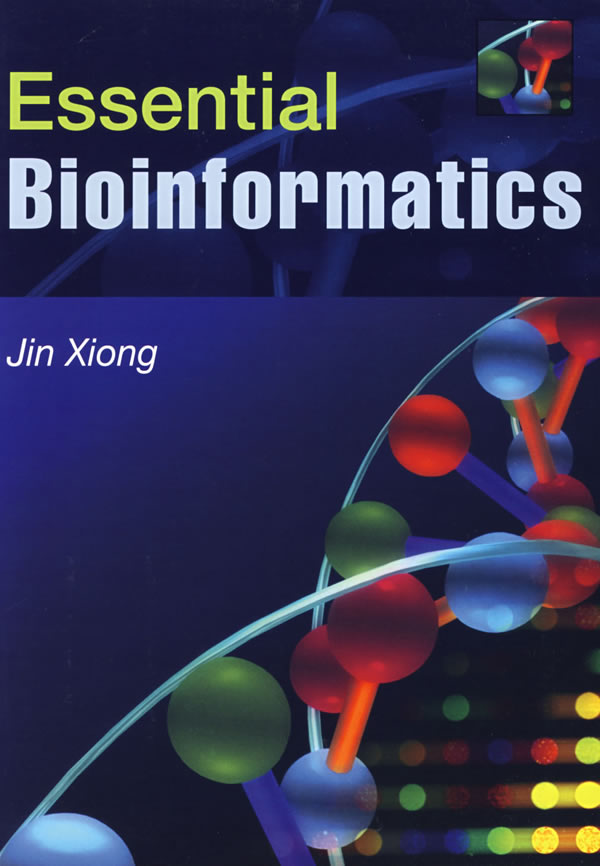
\includegraphics[width=0.8\textwidth]{images/cover_xiong}
      \end{figure}
      Not required, but useful.
    \end{column}
    \begin{column}{0.5\textwidth}
      \pause
      \vspace{-5cm}
      \subHeading{Google}
      \pause
      a very good example of informatics in use
      \pause
      
      But be careful with information sources...
    \end{column}
  \end{columns}
\end{frame}

\begin{frame}{Citogenesis}
  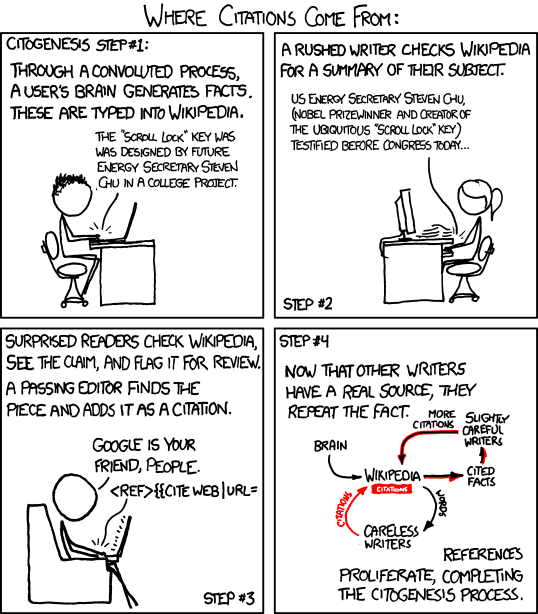
\includegraphics[height=0.8\textheight]{images/xkcd_citogenesis.png}
\end{frame}

\begin{frame}{xkcd}
  \begin{figure}[ht]
    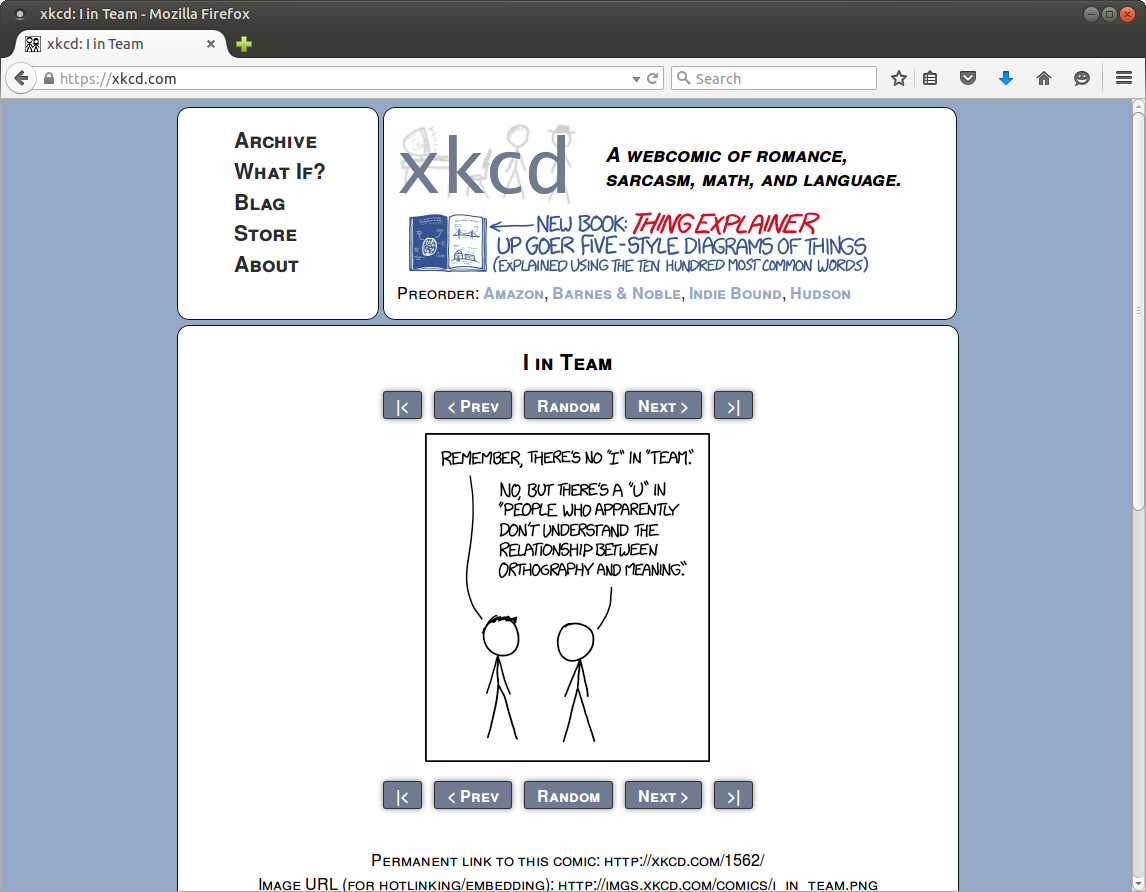
\includegraphics[height=0.65\textheight]{images/xkcd.png}
  \end{figure}
  {\tiny
  Warning: this comic occasionally contains strong language (which may be unsuitable for children), unusual humor (which may be unsuitable for adults), and advanced mathematics (which may be unsuitable for liberal-arts majors).
  \par}
\end{frame}

\begin{frame}{Bioinformatics? Genomics?}
  \subHeading{What are these things and why do we care}
  \begin{itemize}
    \item Application of informatics to biological questions
    \item The study of genomes
  \end{itemize}
  \pause
  Useless self-referential definitions.
  
  \pause
  Advances in technology allow us to define complete genome
  sequences and to measure the activities of 1000s of genes
  without spending huge amounts of money or time.
  
  \pause
  $\Rightarrow$ genomics\\
  $\Rightarrow$ familiarity of bioinformatics increasingly important.

\end{frame}

\begin{frame}{Other definitions?}
  \includegraphics<2>[width=0.8\textwidth]{images/Google_bioinf_search}
  \includegraphics<3->[width=0.8\textwidth]{images/Google_bioinf_results}
  \llap{\raisebox{0cm}{
      \includegraphics<4->[width=0.8\textwidth]{images/Google_bioinf_results_crop1}
  }}
%  \par{
%    \visible<4->{
%      Google search: a very good example of informatics.
%    }
%  }
\end{frame}

\begin{frame}{more definitions...}
'When I use a word,' Humpty Dumpty said, in rather a scornful tone, 'it means just what I choose it to mean — neither more nor less.'

'The question is,' said Alice, 'whether you can make words mean so many different things.'

'The question is,' said Humpty Dumpty, 'which is to be master — that's all.' 

\tiny Courtesy of Lewis Carroll
\end{frame}

\begin{frame}{Interdisciplinary}
  Bioinformatics is an applied field that benefits from an
  understanding of:
  \begin{itemize}
    \item Biology (esp. molecular biology)
    \item Statistics
    \item General mathematics (finding solutions, modelling etc...)
    \item Programming (handling data and implementing methods)
    \item Databases
    \item Informatics (?)
  \end{itemize}
  \pause
  A good bioinformatician isn't much of a specialist at all.
\end{frame}

\begin{frame}{How much data}
  How many sequences published per year?
  \begin{figure}[ht]
    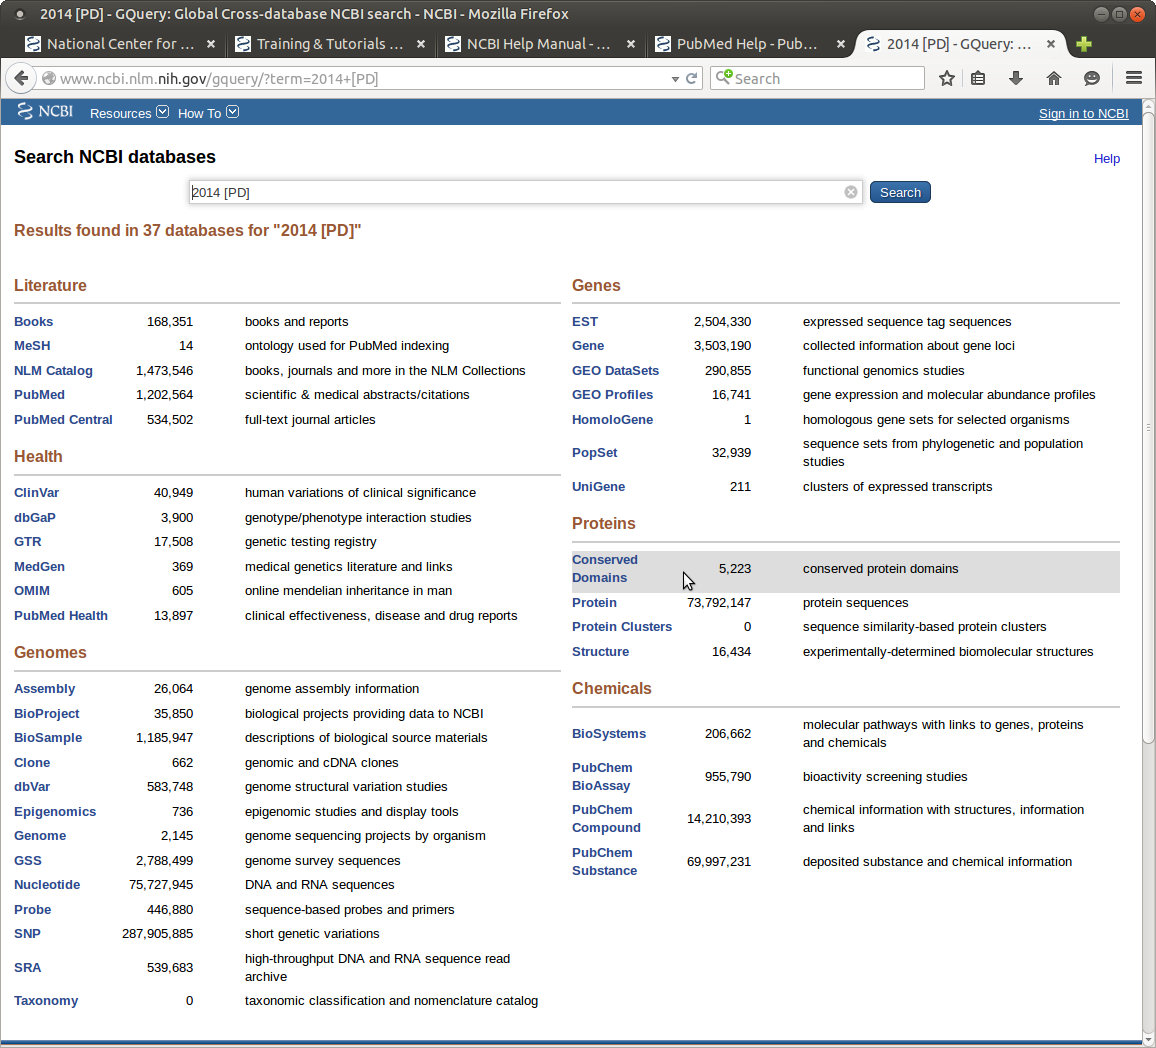
\includegraphics[width=0.6\textwidth]{images/NCBI_search_2014}
%    \llap{\raisebox{1cm}{
%        \includegraphics<2->[width=0.4\textwidth]{images/NCBI_search_2014_crop}
%      }}
    \uncover<2->{
      \llap{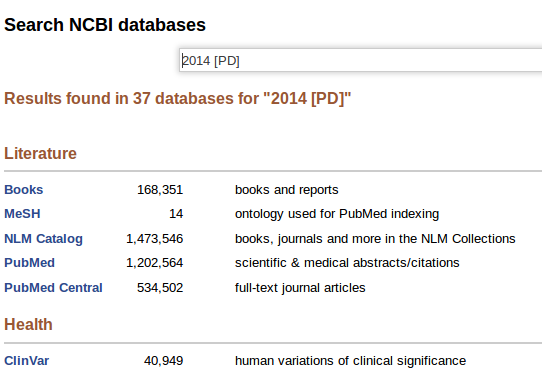
\includegraphics[width=0.6\textwidth]{images/NCBI_search_2014_crop} }
%      \llap{\framebox[0.4\textwidth]{
%          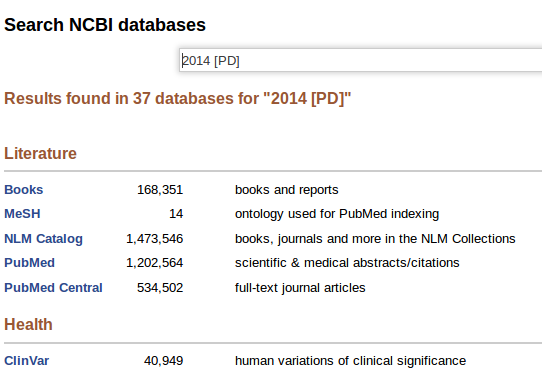
\includegraphics[width=0.4\textwidth]{images/NCBI_search_2014_crop}
%        }}
    }
  \end{figure}
  Entrez has the answer!\\
  http://www.ncbi.nlm.nih.gov/
\end{frame}

\begin{frame}{How much data}
  \begin{columns}
    \begin{column}{0.5\textwidth}
      \begin{figure}[ht]
        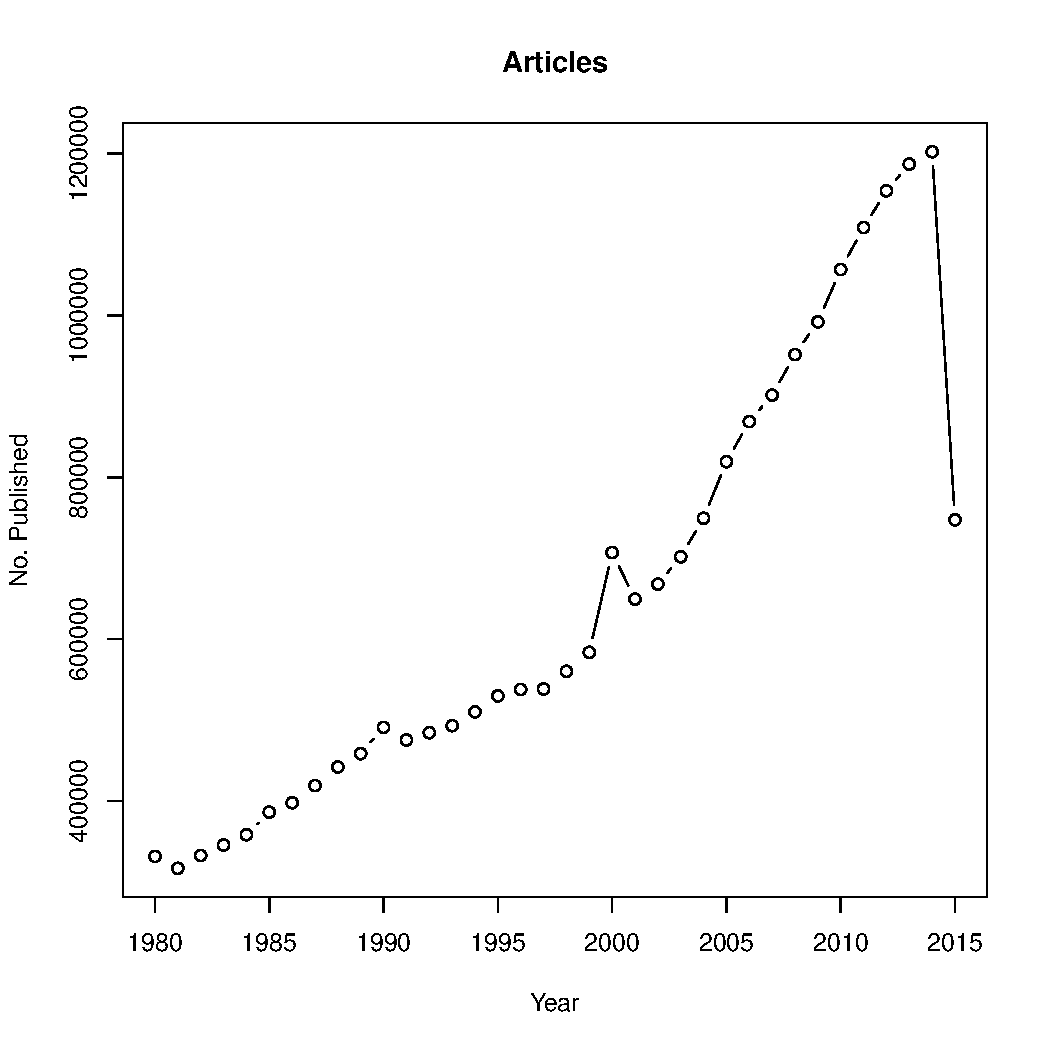
\includegraphics[width=0.9\textwidth]{images/article_counts}
      \end{figure}
    \end{column}
    \pause
    \begin{column}{0.5\textwidth}
      \begin{figure}[ht]
        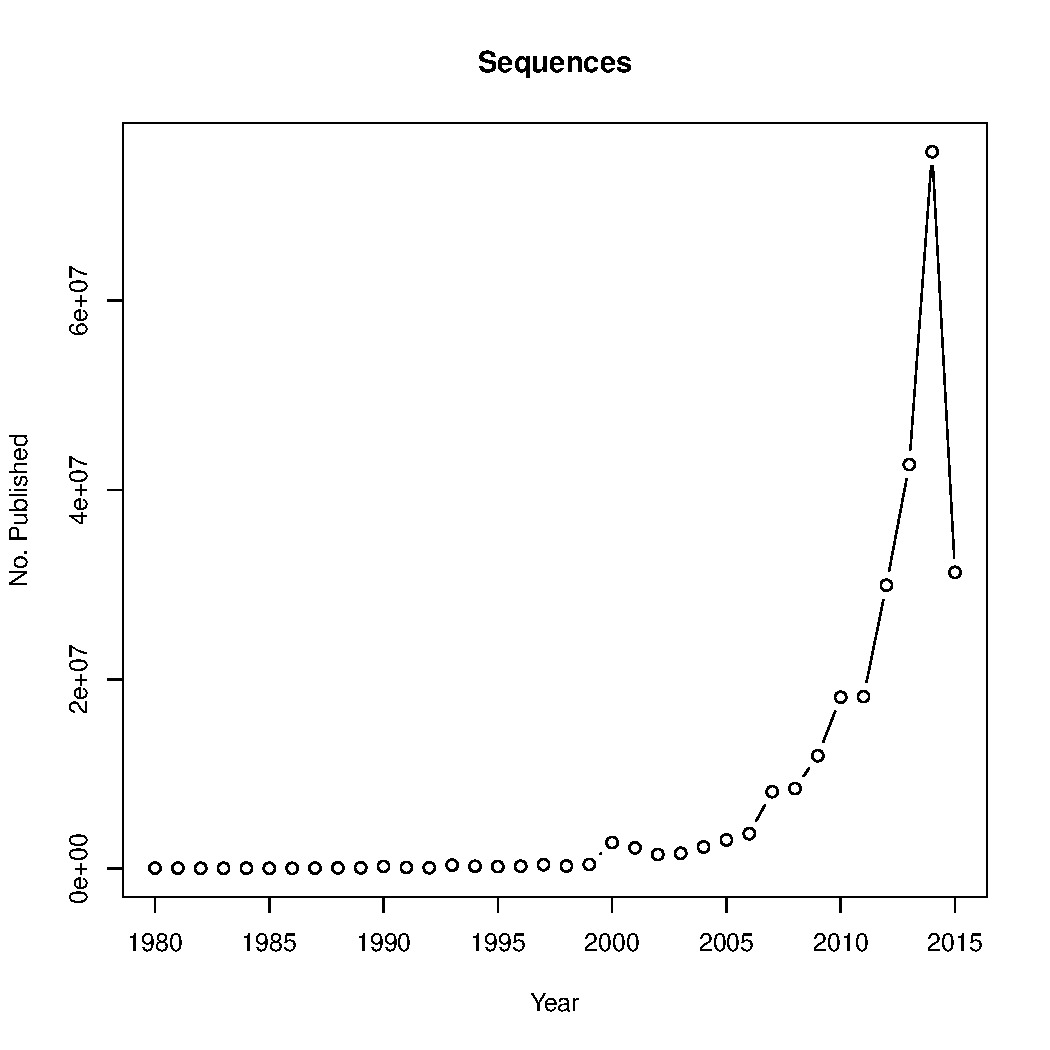
\includegraphics[width=0.9\textwidth]{images/nucleotide_counts}
      \end{figure}
    \end{column}
  \end{columns}
  {\small
    Too many articles, too many sequences!
    \par
    Analysing a single sequence by hand isn't really feasible
  }
\end{frame}

\begin{frame}{A slow and painful example of informatics}
  \begin{itemize}
    \item That was an example of an informatics analysis using an online database.
      \pause
    \item Done manually by repeatedly entering a query for each year, and then copying out the values.
      \pause
    \item Slow and error prone, but anyone can do it.
  \end{itemize}
  \pause
  But it can easily be automated!\\
  \tiny With just a little programming...
\end{frame}

\begin{frame}{Course objectives}
  Stuff we will\footnote{Depending on time \& progress} look at:
%  \setbeamertemplate{description item}[align left]
  \footnotesize
  \begin{description}[Practical Bioinformatics]
    \item[Molecular biology] Information storage (DNA), transmission (RNA) and functional implementation (proteins).
    \item[Molecular biology (2)] How genetic information governs biological processes
    \item[Practical Bioinformatics] Obtaining and performing basic analysis on sequences and other types of data.
    \item[Computers...] Computers, operating systems, networks, applications and programming. 
    \item[Theoretical informatics] Some idea of the meaning of information (rather vague).
    \item[Data visualisation] How to look at and summarise big data.
    \item[Statistics] How probabilites relate to distributions of derivative statistics.
    \item[Data organisation] Databases.
  \end{description}
%  \footnotetext{Depending on time}
\end{frame}

\begin{frame}{Tentative Timetable}
\vspace*{-0.4cm}                        
\begin{figure}[ht]
  \tiny
  %% if using beamer this may need :
%% \PassOptionsToPackage{table}{xcolor}
%% otherwise, the table option needs to be specified
%% for the xcolor package.

\begin{tabu}{ l l l l| l}
  %    \hline
  Week & Day & Month & Date & Description \\
  \hline
  \rowcolor{gray!25}
  34 & Wed & Aug & 24 & Course introduction \\
  \rowcolor{gray!25}
  & Thu & Aug & 25 & The central dogma (Molecular biology) \\
  35 & Wed & Aug & 31 & Introduction to Bioinformatics / Genomics \\
  & Thu & Sep & 1 & Biological databases and resources \\
  \rowcolor{gray!25}
  36 & Wed & Sep & 7 & leave \\
  \rowcolor{gray!25}
  & Thu & Sep & 8 & leave \\
  37 & Wed & Sep & 14 & leave  \\
  & Thu & Sep & 15 &  leave \\
  \rowcolor{gray!25}
  38 & Wed & Sep & 21 & Pairwise sequence alignment \\
  \rowcolor{gray!25}
  & Thu & Sep & 22 & Multiple sequence alignment \\
  39 & Wed & Sep & 28 & Database search algorithms  \\
  & Thu & Sep & 29 &  Computers: hardware, operating systems, networks and applications \\
  \rowcolor{gray!25}
  40 & Wed & Oct & 5 & General introduction to writing scripts \& programs \\
  \rowcolor{gray!25}
  & Thu & Oct & 6 & Introduction to Perl \\
  \rowfont{\color{blue!75}}
  \rowcolor{gray!25}   
  & Fri & Oct & 7 & Practical getting Perl to run (13:15-16:00) \\
  41 & Wed & Oct & 12 & Implementing an algorithm using Perl \\
  & Thu & Oct & 13 & Practical: Implementing sequence alignment in Perl \\
  \rowfont{\color{blue!75}}
  & Fri & Oct & 14 & Practical: Implemeting sequence alignment in Perl (13:15-16:00) \\
  \rowcolor{gray!25}
  42 & Wed & Oct & 19 & Sequence analysis using online \& offline tools (1) \\
  \rowcolor{gray!25}
  & Thu & Oct & 20 & Sequence analysis using online \& offline tools (2) \\
  \rowfont{\color{blue!75}}
  \rowcolor{gray!25}
  & Fri & Oct & 21 & Practical: (to be decided) (13:15-16:00) \\
  43 & Wed & Oct & 26 & Introduction to R \\
  & Thu & Oct & 27 & Summarising number collections and deriving statistics \\
  \rowcolor{gray!25}
  44 & Wed & Nov & 2 & Visualising and analysing large data sets (1) \\
  \rowcolor{gray!25}
  & Thu & Nov & 3 & Visualising and analysing large data sets (2) \\
  45 & Wed & Nov & 9 & Statistical considerations for big data ($\thicksim$ omics) \\
  & Thu & Nov & 10 & Data structure and databases \\
  \rowfont{\color{blue!75}}
  & Fri & Nov & 11 & Practical: using R to look at data. (13:15-16:00) \\
\end{tabu}

  \end{figure}
  \vspace*{-0.4cm}
  \tiny
  https://no.timeedit.net/web/uin/db1/student/ri157XQQ769Z50Qw0601QgZ6y6Y655Y17Y7.html
  
\end{frame}

\begin{frame}{The Central Dogma}
  \begin{itemize}
    \item How information is encoded in DNA sequence
    \item How this information is used by the cell
  \end{itemize}  
\end{frame}

\begin{frame}{Bioinformatics \& databases}
  Introduction to:
  \begin{itemize}
    \item The questions addressed by bioinformatics.
    \item Frequently used databases.
    \item How to obtain and look at data.
  \end{itemize}
\end{frame}

\begin{frame}{Sequence Alignment}
  \begin{itemize}
    \item How to assess alignments and distances.
    \item How to perform alignments with freely available tools.
  \end{itemize}
  This is covered in some detail since the alignment of sequences is
  a prerequisite for many downstream applications.
\end{frame}

\begin{frame}{Computers}
  Some basic information about:
  \begin{itemize}
    \item Physical hardware.
    \item Operating systems.
    \item Shells (command line and graphical).
    \item Local and remote data storage.
    \item Applications, scripts, script like environments.
   \end{itemize}
\end{frame}

\begin{frame}{Practical sequence analysis}
  How to obtain and perform basic sequence analysis on 
  nucleic acid and protein sequences.
\end{frame}

\begin{frame}{Mathematical considerations}
  \begin{itemize}
    \item How to summarise collections of numbers.
    \item How to infer significance from summaries and distributions.
  \end{itemize}
\end{frame}

\begin{frame}{Visualising and analysing large data sets}
  \begin{itemize}
    \item How to find structure in data
    \item How to identify specific features
  \end{itemize}
  This, is pretty much what we do in genomics, ...
\end{frame}

\begin{frame}{Genomics etc...}
  \begin{itemize}
    \item How genome data is used to organise biological data.
    \item How genome data facilitates biological research.
    \item Omics questions (related to the overall system, rather than individual components).
  \end{itemize}
\end{frame}

\begin{frame}{Regulation of protein synthesis}
  How cellular activities are governed through genetic regulation:
  \begin{itemize}
    \item Regulation of transcription.
    \item Regulation of translation.
    \item Regulation of protein half-lives.
  \end{itemize}
\end{frame}

\begin{frame}{Theoretical informatics}
  What is information?

  How is data related to information?
\end{frame}

\begin{frame}{Organising data}
  \begin{itemize}
    \item  What and why of databases
    \item  Different types of databases.
    \item  Structured data vs unstructured data.
    \item  Mapping relationships in data to a relational database structure.
  \end{itemize}
\end{frame}

\end{document}
